\documentclass[12pt,a4paper]{article}
\usepackage[utf8]{inputenc}
\usepackage[T1]{fontenc}
\usepackage[french]{babel}
\usepackage{graphicx}
\usepackage{geometry}
\geometry{margin=2cm}
\usepackage{multicol}
\setlength{\parskip}{0.5em}
\setlength{\parindent}{0pt}

\title{Architecture d'une Plateforme IA -- DeepSeek}
\author{Yosr Barghouti}
\date{\today}

\begin{document}

\maketitle

\section*{Introduction}
Ce rapport décrit l’architecture d’une plateforme IA type \textbf{DeepSeek}. L’objectif est de présenter les composants principaux et les mécanismes de résilience tout en restant concis pour tenir sur 2 pages.

\section*{Architecture Globale}
La plateforme suit une architecture en couches :
\begin{itemize}
    \item \textbf{Data Layer} : ingestion, prétraitement et gouvernance.
    \item \textbf{Training} : clusters GPU/TPU, entraînement distribué.
    \item \textbf{Model Layer} : LLM, fine-tuning, sécurité et alignment.
    \item \textbf{Serving} : microservices d’inférence, optimisation et routage.
    \item \textbf{Application} : SDKs, intégrations, produits finaux.
    \item \textbf{Monitoring} : observabilité, sécurité et conformité.
\end{itemize}

\section*{Data Layer}
Collecte multi-sources (texte, code, multimodal), prétraitement (nettoyage, tokenisation), stockage distribué (data lake, S3) et gouvernance (audit, conformité RGPD).

\section*{Model Training}
Clusters GPU/TPU, frameworks distribués (DeepSpeed, Megatron), hyperparamètres, checkpoints et suivi de l’expérimentation.

\section*{Model Layer}
LLMs et modèles multimodaux, fine-tuning (RLHF, DPO), filtres de sécurité et red-teaming pour réduire les biais.

\section*{Serving \& Microservices}
Chaque service critique est isolé :
\begin{itemize}
    \item Auth, Rate Limiting
    \item Billing \& Quotas
    \item Model Routing
    \item Inference clusters (Primary / Fallback)
    \item Fine-tuning
    \item Logging \& Monitoring
    \item Moderation
\end{itemize}

\section*{API Gateway et Patterns de Résilience}
- Authentification et quotas  
- Circuit breaker et retry  
- Routage Primary $\rightarrow$ Fallback $\rightarrow$ Cache  
- Cache-Aside (Redis/Vector DB)  
- Bulkhead et Rate Limiting  

\section*{Fallback Architecture}
Ordre de résolution :
\begin{enumerate}
    \item Primary Inference Service (modèle principal)
    \item Fallback Inference Service (modèle plus petit)
    \item Cache Layer (résultats chauds)
    \item Erreur structurée si tout échoue (503)
\end{enumerate}

\section*{Monitoring \& Compliance}
Observabilité via Prometheus/ELK/Jaeger, chiffrement TLS, IAM, RBAC, conformité RGPD, safety filters et red-teaming.

\section*{Diagramme Simplifié}
\begin{center}
    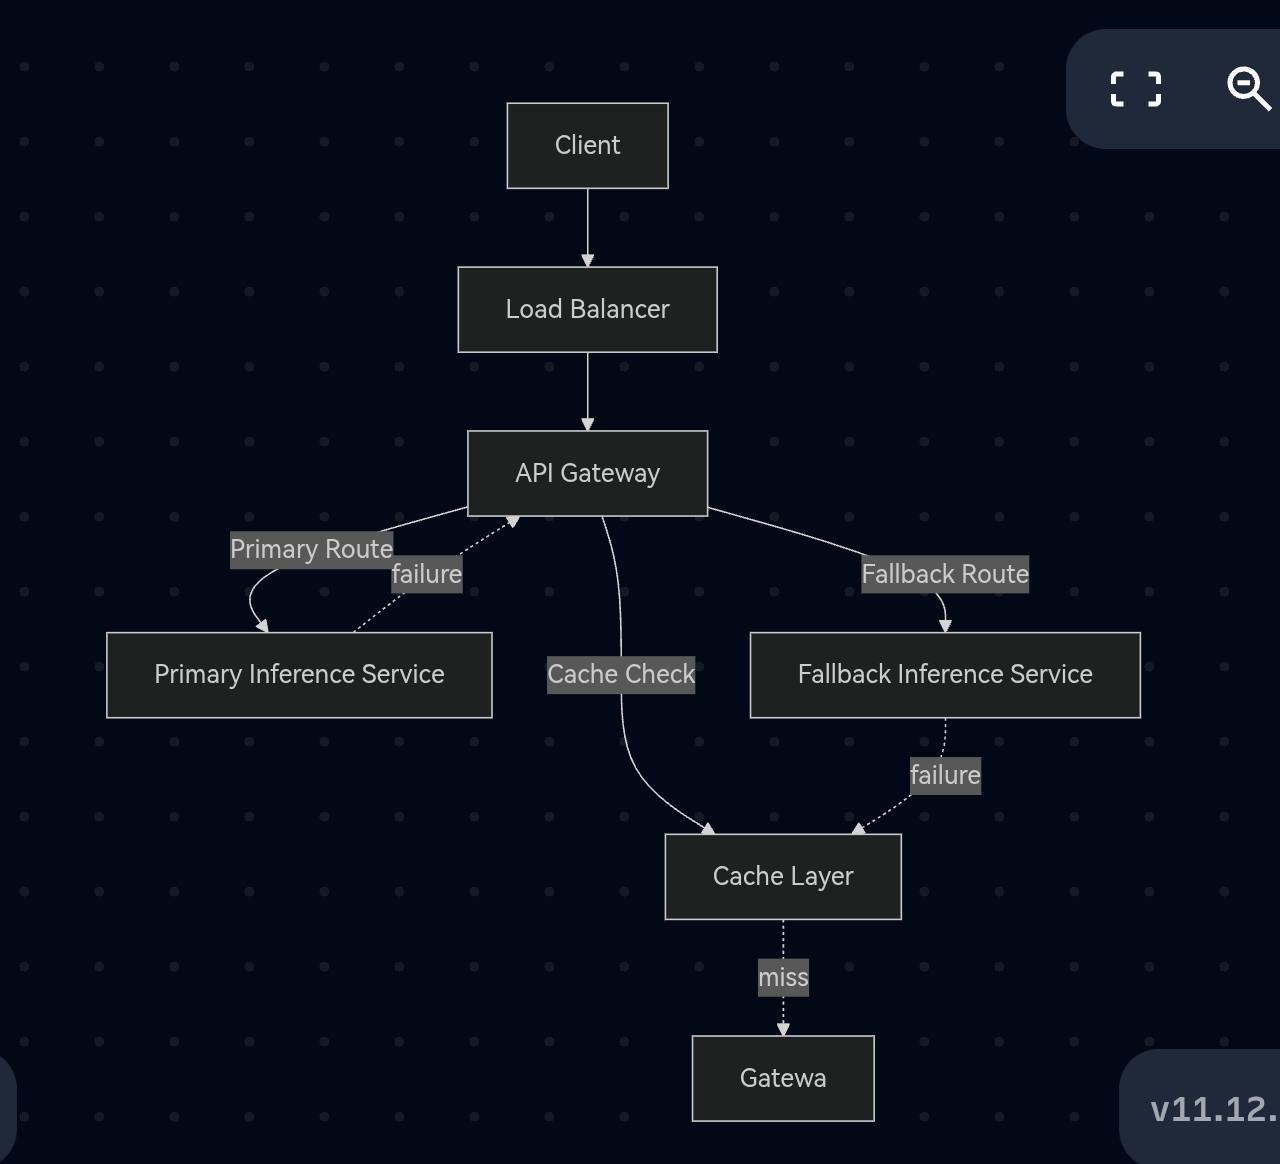
\includegraphics[width=0.9\textwidth]{mermaid.jpg}
\end{center}

\section*{Conclusion}
L’architecture modulaire permet de :
\begin{itemize}
    \item Monter en charge (scalabilité horizontale)
    \item Tolérance aux pannes via fallback, circuit breaker, cache
    \item Sécurité et conformité
    \item Exposer des APIs robustes aux développeurs
\end{itemize}

\end{document}